%%%%%%%%%%%%%%%%%%%%%%%%%%%%%%%%%%%%%%%%%%%%%%%%%%%%%%%%%%%%%%%%%%%%%%%%%%%%%%%%
% Copyright 2019-2022 Louis Paternault --- http://snt.ababsurdo.fr
%
% Publié sous licence Creative Commons Attribution-ShareAlike 4.0 International (CC BY-SA 4.0)
% http://creativecommons.org/licenses/by-sa/4.0/deed.fr
%%%%%%%%%%%%%%%%%%%%%%%%%%%%%%%%%%%%%%%%%%%%%%%%%%%%%%%%%%%%%%%%%%%%%%%%%%%%%%%%

% Pour compiler :

%$ lualatex $basename
%$ pdftoppm -png $basename.pdf $basename

\documentclass[tikz]{standalone}

\begin{document}
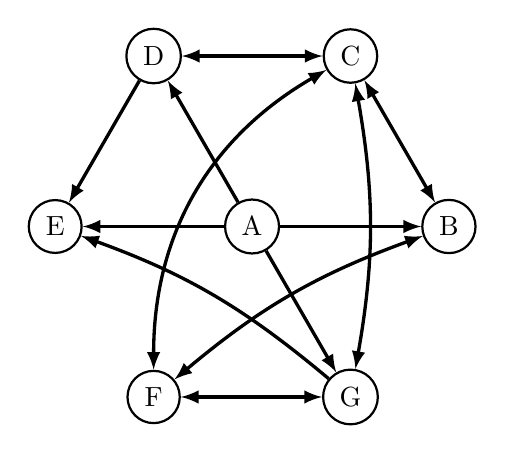
\begin{tikzpicture}[scale=1,very thick]
  \begin{scope}[every node/.style={circle,thick,draw,fill=white}]
    \node (A) at (0,0) {A};
    \node (B) at (00:2.5) {B};
    \node (C) at (60:2.5) {C};
    \node (D) at (120:2.5) {D};
    \node (E) at (180:2.5) {E};
    \node (F) at (240:2.5) {F};
    \node (G) at (300:2.5) {G};
  \end{scope}

  \begin{scope}
    \draw[-latex] (A) edge (B) edge (D) edge (E) edge (G);
    \draw[-latex] (D) edge (E);
    \draw[-latex] (G) edge[bend right=10] (E);
    \draw[latex-latex] (C) edge (B) edge[bend right] (F) edge[bend left=10] (G);
    \draw[latex-latex] (D) edge (C);
    \draw[latex-latex] (B) edge[bend right=10] (F);
    \draw[latex-latex] (G) edge (F);
  \end{scope}
\end{tikzpicture}

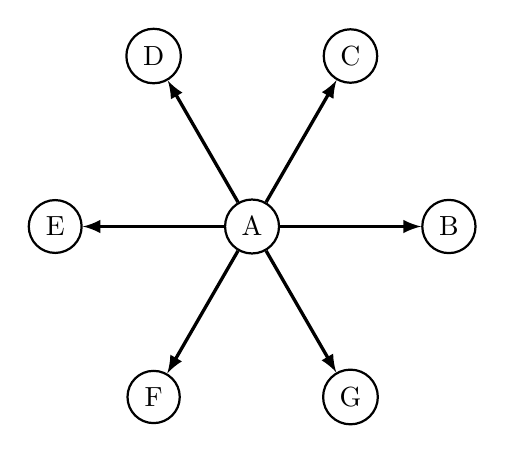
\begin{tikzpicture}[scale=1,very thick]
  \begin{scope}[every node/.style={circle,thick,draw,fill=white}]
    \node (A) at (0,0) {A};
    \node (B) at (00:2.5) {B};
    \node (C) at (60:2.5) {C};
    \node (D) at (120:2.5) {D};
    \node (E) at (180:2.5) {E};
    \node (F) at (240:2.5) {F};
    \node (G) at (300:2.5) {G};
  \end{scope}

  \foreach \sommet in {B, C, D, E, F, G} {
    \path [-latex] (A) edge  (\sommet);
  }
\end{tikzpicture}

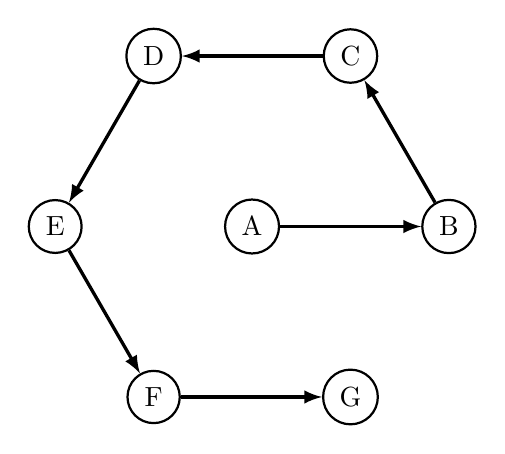
\begin{tikzpicture}[scale=1,very thick]
  \begin{scope}[every node/.style={circle,thick,draw,fill=white}]
    \node (A) at (0,0) {A};
    \node (B) at (00:2.5) {B};
    \node (C) at (60:2.5) {C};
    \node (D) at (120:2.5) {D};
    \node (E) at (180:2.5) {E};
    \node (F) at (240:2.5) {F};
    \node (G) at (300:2.5) {G};
  \end{scope}

  \draw[-latex] (A) --  (B);
  \draw[-latex] (B) --  (C);
  \draw[-latex] (C) --  (D);
  \draw[-latex] (D) --  (E);
  \draw[-latex] (E) --  (F);
  \draw[-latex] (F) --  (G);
\end{tikzpicture}

\end{document}
